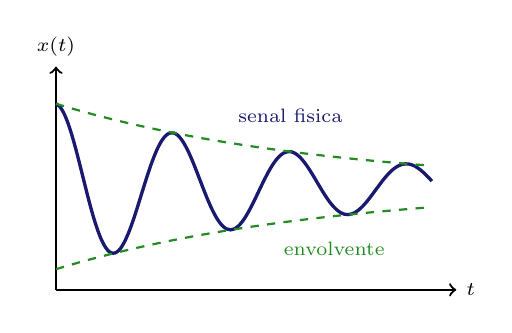
\begin{tikzpicture}[x=0.62cm,y=1.05cm]
\draw[->,thick] (0,-1.25) -- (8.2,-1.25) node[right,font=\scriptsize] {$t$};
\draw[->,thick] (0,-1.25) -- (0,1.45) node[above,font=\scriptsize] {$x(t)$};
\draw[very thick,MidnightBlue] plot[smooth,samples=100,domain=0:7.7] (\x,{exp(-0.18*\x)*cos(150*\x)});
\draw[dashed,ForestGreen,thick] plot[smooth,samples=80,domain=0:7.7] (\x,{exp(-0.18*\x)});
\draw[dashed,ForestGreen,thick] plot[smooth,samples=80,domain=0:7.7] (\x,{-exp(-0.18*\x)});
\node[font=\scriptsize,MidnightBlue] at (4.8,0.85) {senal fisica};
\node[font=\scriptsize,ForestGreen] at (5.7,-0.75) {envolvente};
\end{tikzpicture}
